\chapter{Desenvolvimento}
\label{chapter:desenvolvimento}

Neste capítulo, são apresentadas a contribuição deste trabalho. Na Seção \ref{sec:metodologia} é apresentada a metodologia utilizada para a coleta e processamento dos dados. Na Seção \ref{sec:resultados} são apresentados os resultados encontrados na abordagem.

\section{Metodologia Utilizada} \label{sec:metodologia}

%Foi planejado e realizado um estudo que visa avaliar estado manutenibilidade
%do Linux Kernel, utilizando o sofware SonarQube para a medição. Os
%requerimentos necessários pelo método SQALE foram as fornecidas pelo
%plugin \textbf{sonar-cxx\cite{Sonarcxx2016}}. O software realiza
%uma leitura completa do código fonte da aplicação a ser analisada,
%identificando os trechos não adequados de acordo com os requerimentos
%definidos. Para cada não conformidade encontrada, há uma função de
%remediação definida com o tempo estimado de remediação cada ocorrência
%encontrada. Foram consideradas 6 versões de lançamento estáveis foram
%analisadas dentro das versões mais recentes, procurando avaliar o
%estado atual da manutenibilidade do software. 
Nesta seção, é apresentada a metodologia utilizada para coleta e análise dos dados. Foram utilizamos os repositórios da \textit{Apache Software Foundation}, onde o código fonte dos \textit{softwares} é armazenado, através do sistema de controle de versão \textit{Git}\footnote{Disponível em https://git-scm.com/}. O \textit{software Git} permite que configurações do projeto(código fonte, arquivos de configuração, artefatos) sejam salvos(em \textit{commits}), mantendo um histórico do estado de todo o projeto ao longo da sua evolução. 

Nele, marcações (\textit{tags}) podem ser criadas para referenciar uma determinada versão. Tais marcações são utilizadas para sinalizar versões de lançamento. Para descrever a evolução do software, um número de versão é geralmente utilizado, contendo três componentes: versão principal(\textit{major version}), versão secundária(\textit{minor version}) e versão de manutenção, separados por pontos (ex: 1.0.0).  Apesar de não existir um padrão unificado para a nomenclatura dos lançamentos(e.g. no Hadoop, as versões são marcadas como \textit{release-X.X.X}, enquanto no Maven são marcadas como maven-X.X.X), os projetos incluem o número da versão nas marcações. De cada projeto, foram analisadas todas as versões marcadas como lançamentos em que o número da versão não fosse inferior ao atual, evitando assim que as analises fossem realizadas em versões de manutenção, que possuem evolução paralela. Um simples exemplo é apresentado na figura \ref{fig:selecaoversoes}.
\begin{figure}[h]
	\centering
	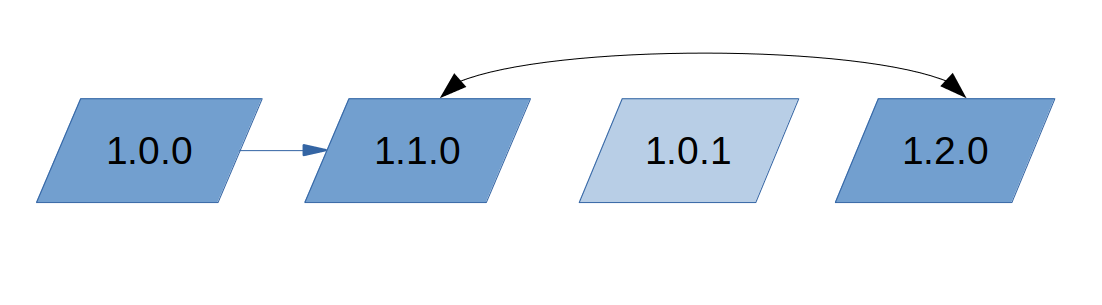
\includegraphics[width=0.7\linewidth]{figure/selecao_versoes}
	\caption{}
	\label{fig:selecaoversoes}
\end{figure}
Como teste preliminar, usaremos o Hadoop, desenvolvido pela Apache Foundation e largamente utilizado. Foram analisadas as versões de lançamento sequências do software. As métricas mostradas são presentadas como uma função do tempo, assim como adotado em \cite{israeli2010linux}, devido a grande variância de lançamento de versões menores. Por exemplo, uma versão nomeada "2.1.1" pode ser lançada após o lançamento de uma versão "3.0.0". Portanto, utilizar as métricas como funções de números de versões pode levar a resultados enganosos.


\section{Resultados e Discussão} \label{sec:resultados}

Nesta seção analisamos as Leis de Evolução de Software de Lehman usando como base dados obtidos do Apache Hadoop. Para cada lei, foram formuladas hipóteses para serem verificadas diante dos dados obtidos, assim como formulado em \cite{neamtiu2013towards}.

\subsection{Lei 1: Mudança Contínua}
Esta Lei determina que o software deve se adaptar constantemente, caso contrário torna-se obsoleto. Os projetos analisados são ativamente mantidos e largamente utilizados, portanto, se a lei é valida, deve-se observar que o programa está em constante mudança. Para caracterizar mudança, foi utilizado o número de adições e remoções em linas de código do projeto. 
\begin{hypothesis}
	O número de mudanças cumulativas em cada release é diferente de zero.
\end{hypothesis}
\begin{figure}[h]
	\centering
	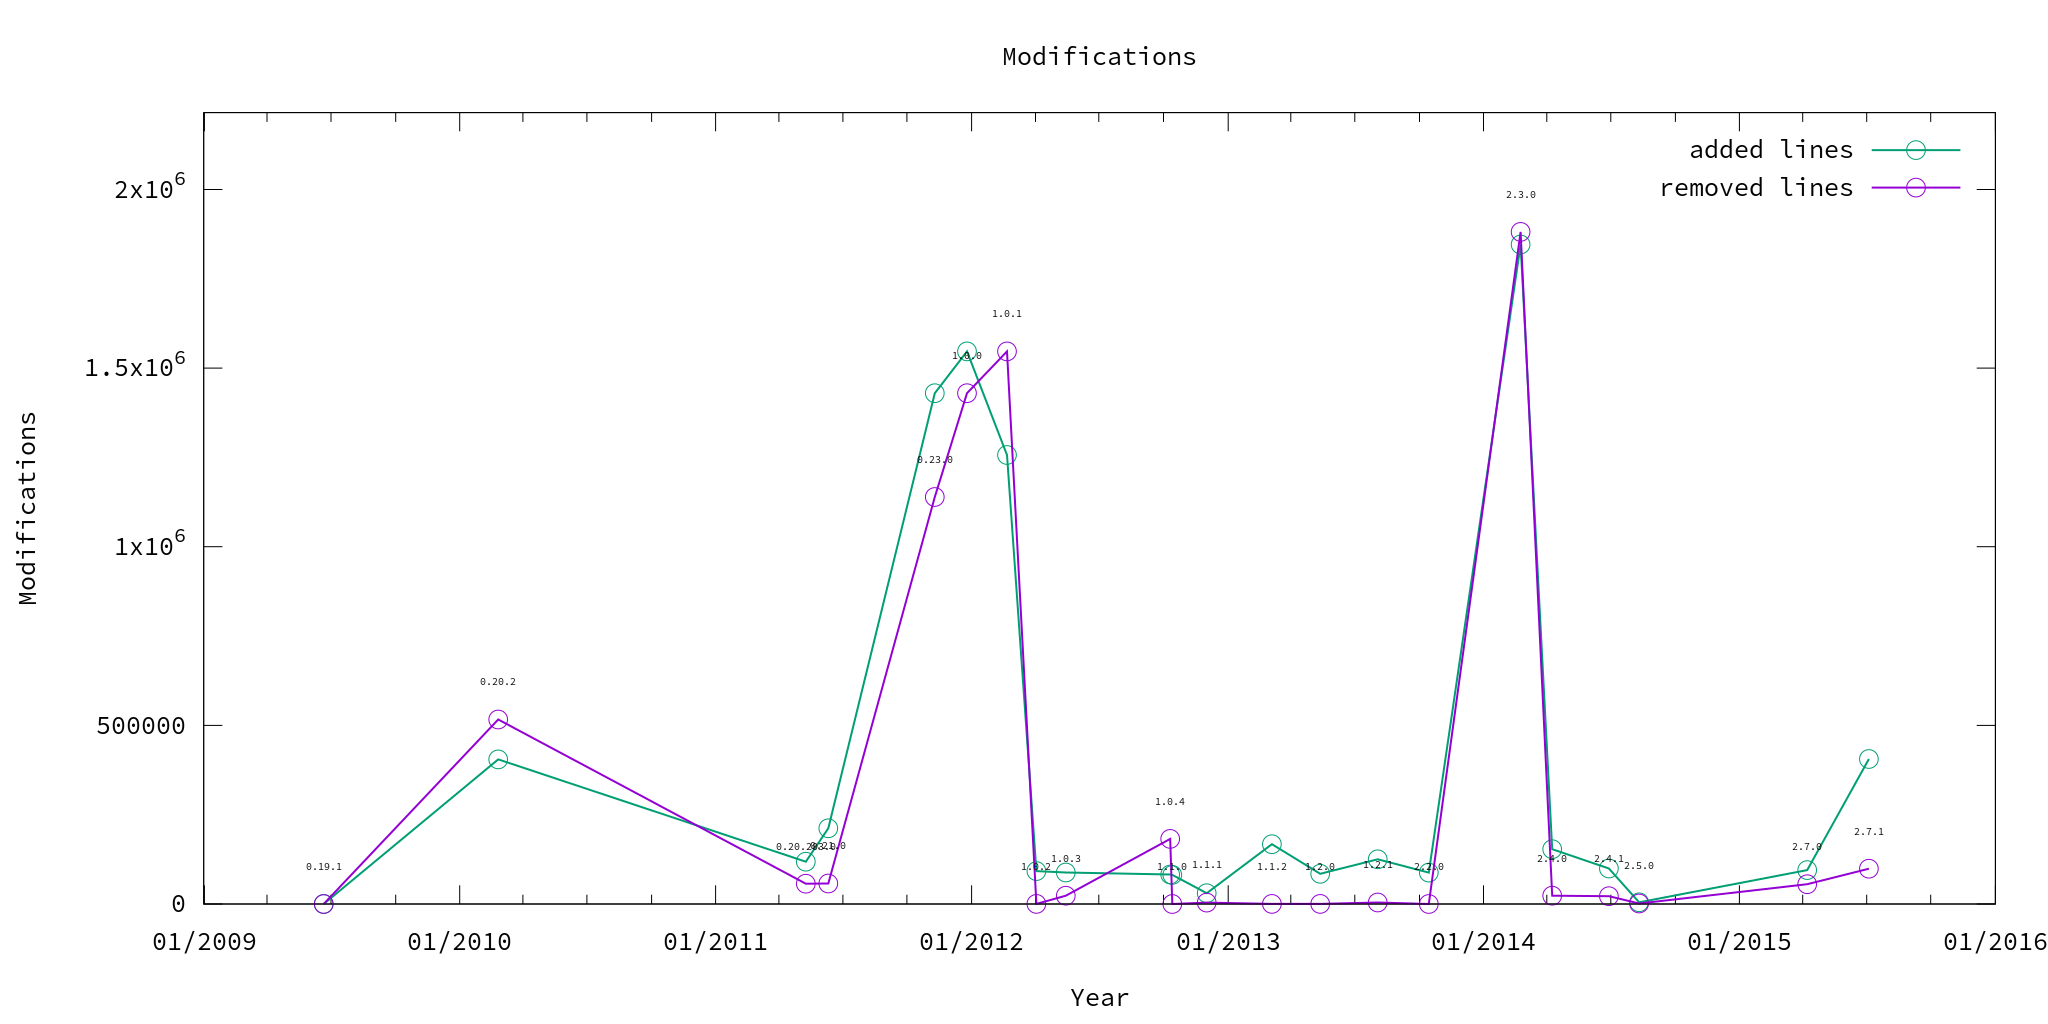
\includegraphics[width=0.9\linewidth]{figure/Modifications}
	\caption{Mudanças no software ao longo do tempo}
	\label{fig:modifications}
\end{figure}
O gráfico da figura \ref{fig:modifications} mostra a evolução das adições e remoções de linhas no projeto. Linhas que foram modificadas, são contabilizadas como uma remoção e uma adição. Observa-se que salvo alguns pontos, o número de linhas adicionadas é superior ao de linhas removidas, o que é esperado se o projeto tende a incorporar novas funcionalidades.

Portanto, verifica-se que a primeira Lei de Lehman é confirmada.

\subsection{Lei 2: Complexidade Crescente}
A segunda lei postula que a medida que um programa cresce, sua complexidade aumenta se não forem realizadas medidas para prevenir tal fato. Para medição da complexidade do código, foi utilizada como métrica a complexidade ciclomática, assim como definida na Seção \ref{subsec:complexidade_ciclomatica}, assim como utilizado em estudos anteriores \cite{israeli2010linux,neamtiu2013towards,skoulis2014open}.
Foram tomadas as seguintes hipóteses:
\begin{hypothesis}
	A complexidade ciclomática total aumenta com o tempo.
\end{hypothesis}
\begin{hypothesis}
	A complexidade ciclomática relativa aumenta com o tempo.
\end{hypothesis}

Como a complexidade total do projeto é afetada pelo seu tamanho, precisamos avaliar também se a complexidade relativa do código cresce ao longo do tempo, isto é, se novas adições tendem a aumentar a complexidade do código em relação ao seu tamanho. As figuras \ref{fig:file_complexity} e \ref{fig:functioncomplexity} mostram respectivamente a complexidade relativa número de arquivos e ao número de funções do código.
\begin{figure}[h]
	\centering
	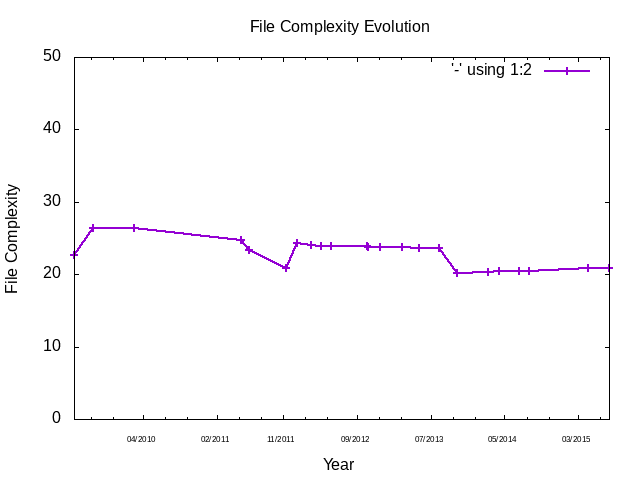
\includegraphics[width=0.7\linewidth]{figure/file_complexity}
	\caption{Evolução da complexidade/Arquivo}
	\label{fig:file_complexity}
\end{figure}
\begin{figure}[h]
	\centering
	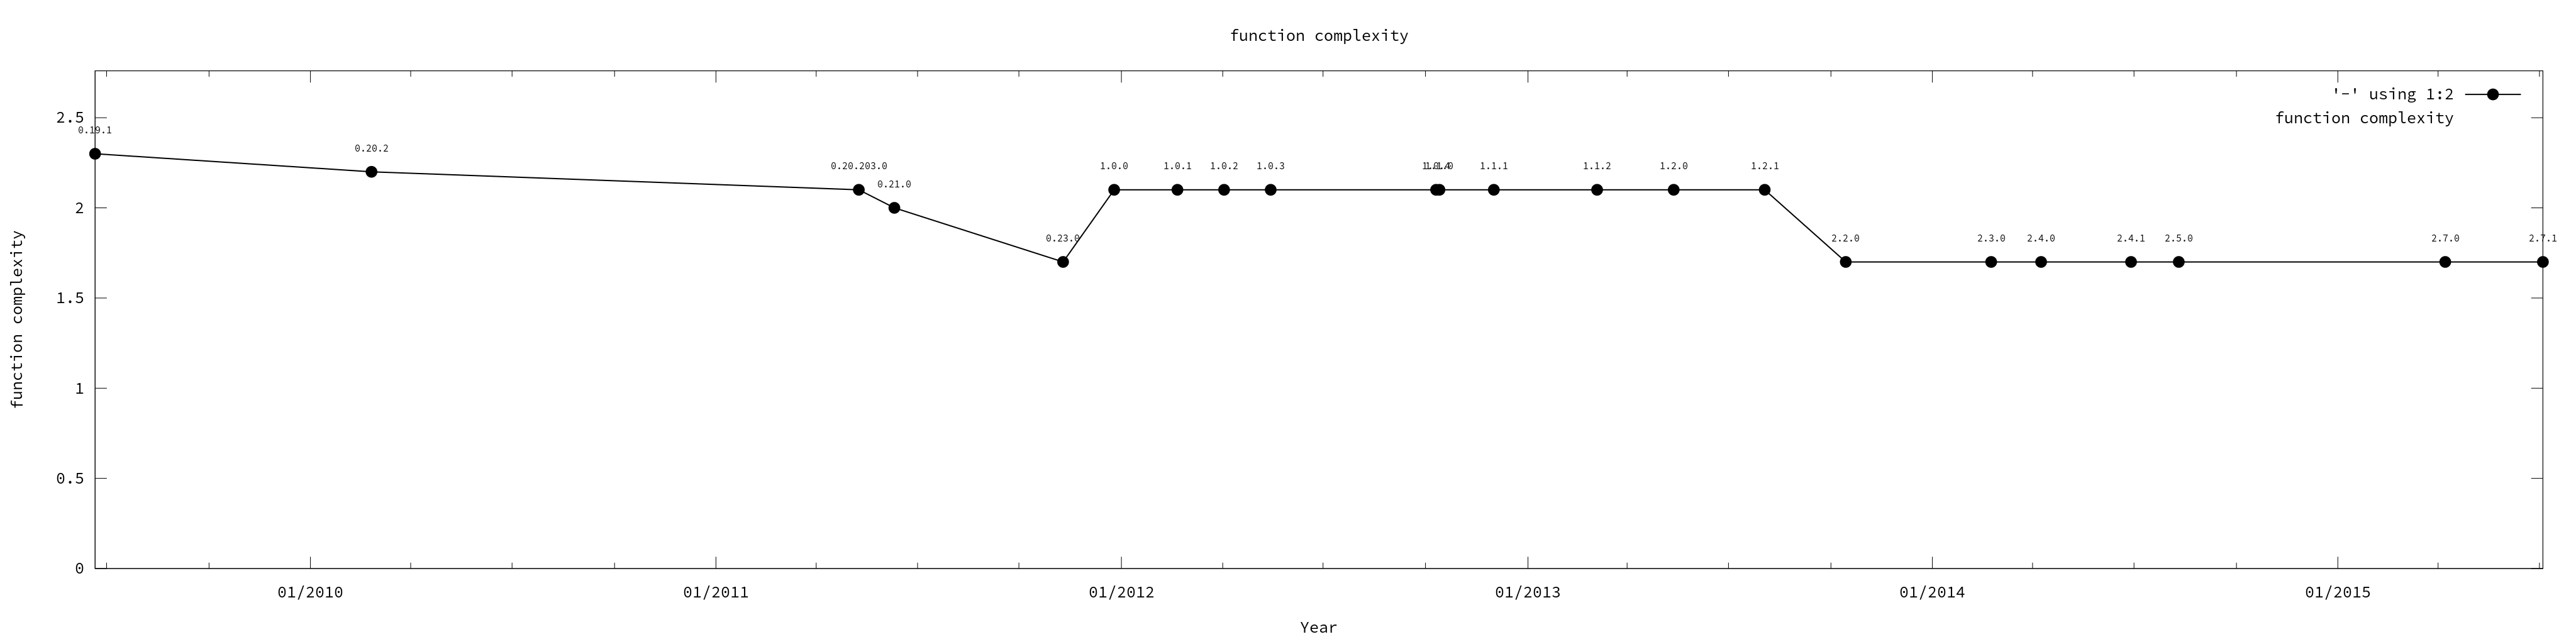
\includegraphics[width=0.7\linewidth]{figure/function_complexity}
	\caption{Evolução da complexidade ciclomática/Função}
	\label{fig:functioncomplexity}
\end{figure}
\begin{figure}[h]
	\centering
	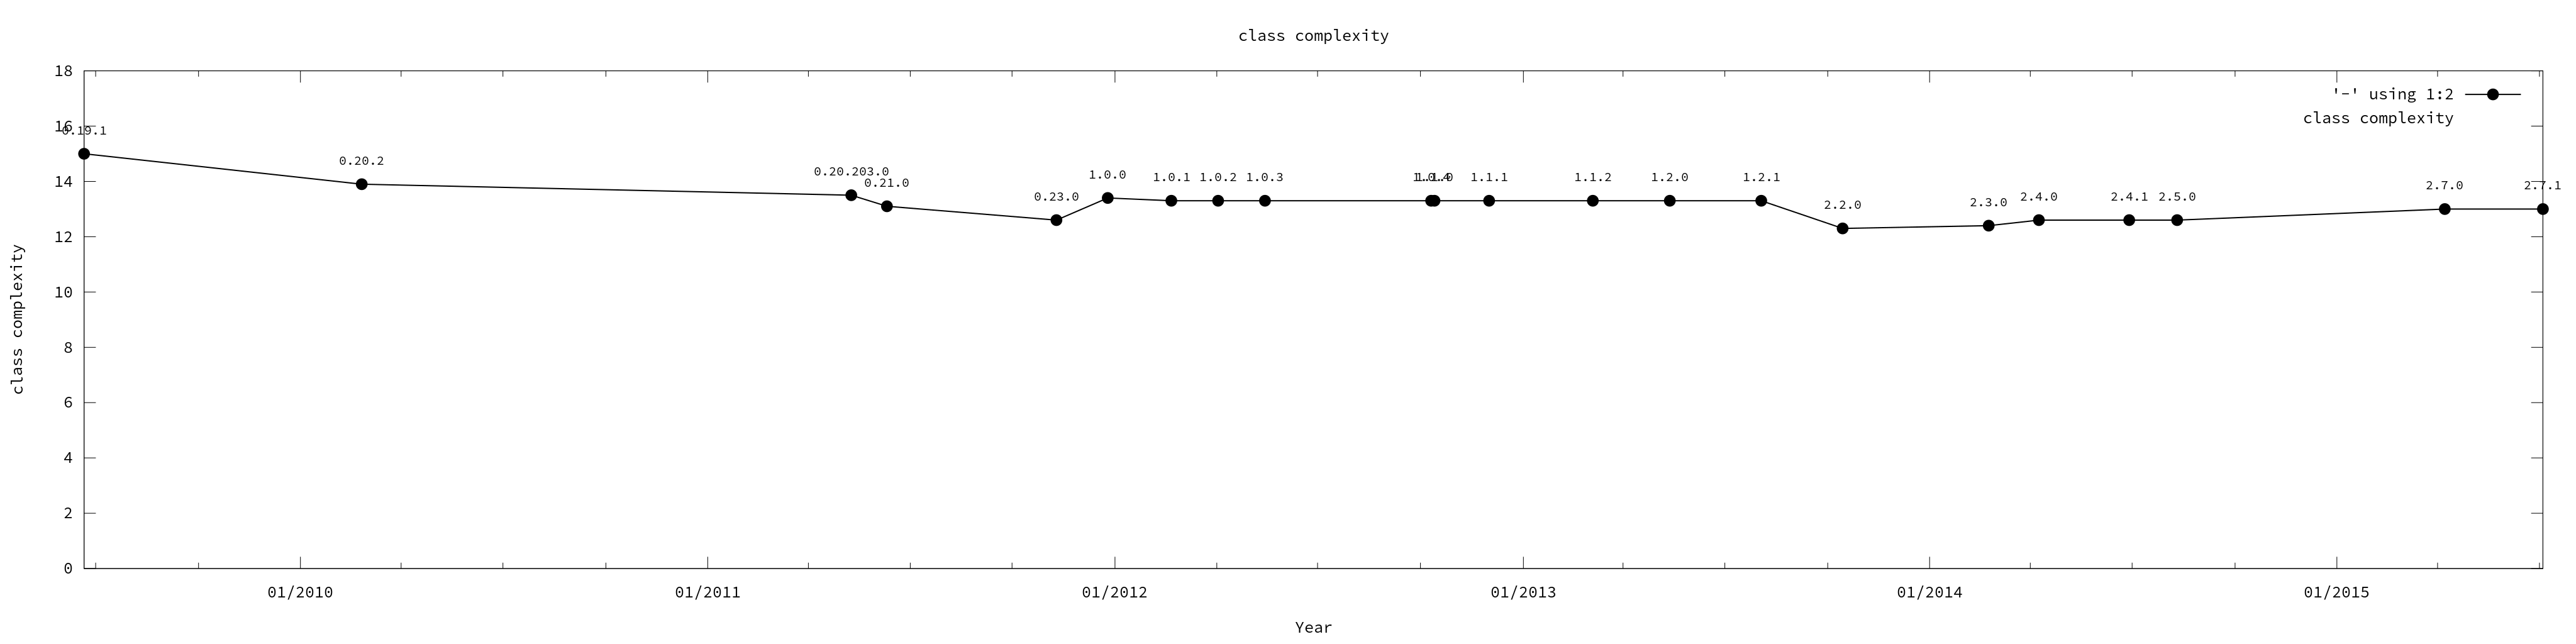
\includegraphics[width=0.7\linewidth]{figure/class_complexity}
	\caption{Evolução da complexidade ciclomática/Classe}
	\label{fig:classcomplexity}
\end{figure}
Pode-se observar que a complexidade possui uma relação com o tamanho total do projeto. Porém, ao contrário do esperado pela segunda Lei de Lehman, a complexidade total do código tende a medida que o projeto evolui. Lehman argumenta que a complexidade aumenta ao longo do tempo, a não ser que esforço seja feito para conter seu avanço. Porém, não é evidente que na evolução do Hadoop houveram esforços focados no controle da condição, sugerindo que o projeto evolui com trabalho constante na amenização da complexidade.

Portanto, pode-se a afirmar que a Segunda Lei de Lehman é falsa para o Hadoop.

\subsection{Lei 3: Auto-Regulação}
Lehman esta lei sugere que a evolução de um grande \textit{sistema} de software é auto-regulado, ajustando seu tamanho ao longo do tempo apresentando adições positivas e negativas de tamanho. Assim, o software deve apresentar tanto ajustes positivos, quanto negativos nas tendências de crescimento do software. Para verificar esta lei, observamos o crescimento incremental de classes e funções no projeto. Portanto, nossas hipóteses são:
\begin{hypothesis}
	O número de lançamentos com ajustes negativos ao número de funções é diferente de zero.
\end{hypothesis}
\begin{hypothesis}
	O número de lançamentos com ajustes negativos ao número de classes é diferente de zero.
\end{hypothesis}

\begin{figure}
	\centering
	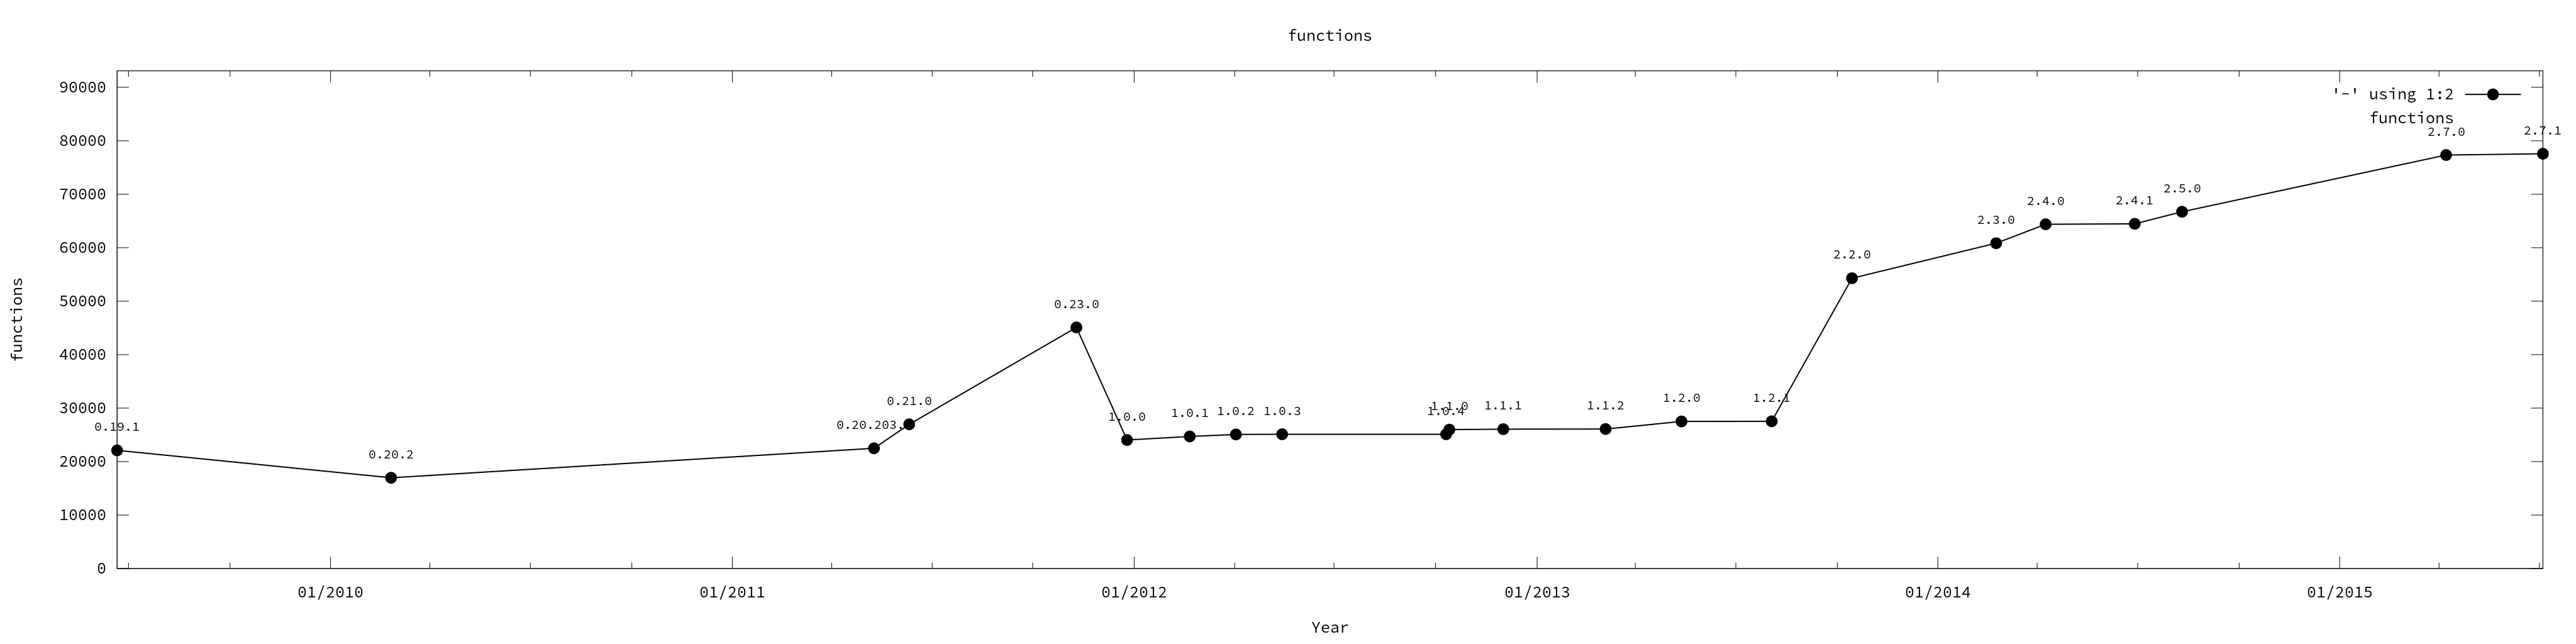
\includegraphics[width=0.7\linewidth]{figure/functions}
	\caption{Crescimento em número de funções}
	\label{fig:function_growth}
\end{figure}

\begin{figure}
	\centering
	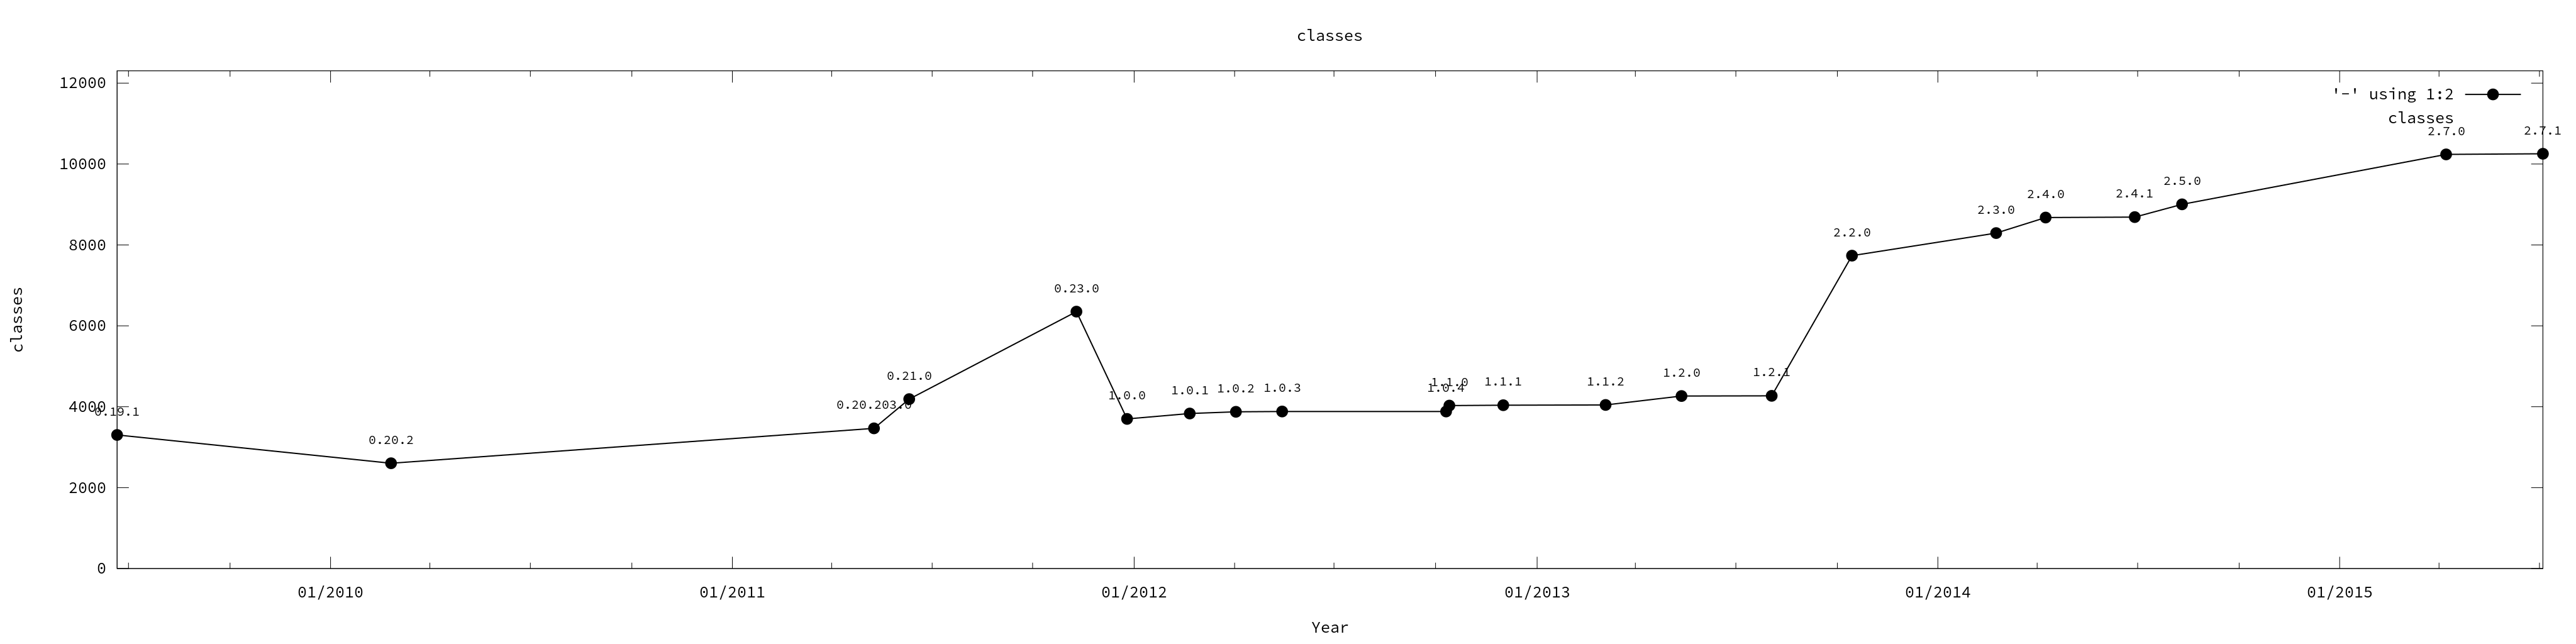
\includegraphics[width=0.7\linewidth]{figure/classes}
	\caption{Crescimento em número de funções}
	\label{fig:classes_growth}
\end{figure}

Nas Figuras \ref{fig:function_growth} e \ref{fig:classes_growth} pode-se representa o crescimento do número de funções e classes,  respectivamente. Pode-se observar que incrementos positivos são mais frequentes do que decrementos, mas ambos estão presentes.

Portanto, pode-se concluir que a Lei de Auto-Regulação é verdadeira.


\subsection{Lei 4: Conservação da estabilidade Organizacional}
Esta lei, também conhecida como "taxa de trabalho invariante" estabelece que o ritmo de trabalho no ciclo de vida do software tende a permanecer constante durante a evolução do projeto. Como utilizado em \cite{neamtiu2013towards}, tomamos como definição de taxa de trabalho o número médio de mudanças realizadas por dia. Assim, nossas hipóteses são:
\begin{hypothesis}
	O número de médio de mudanças por dia é invariante.
\end{hypothesis}

\begin{hypothesis}
	O número de médio de mudanças por dia é invariante.
\end{hypothesis}
\begin{figure}
	\centering
	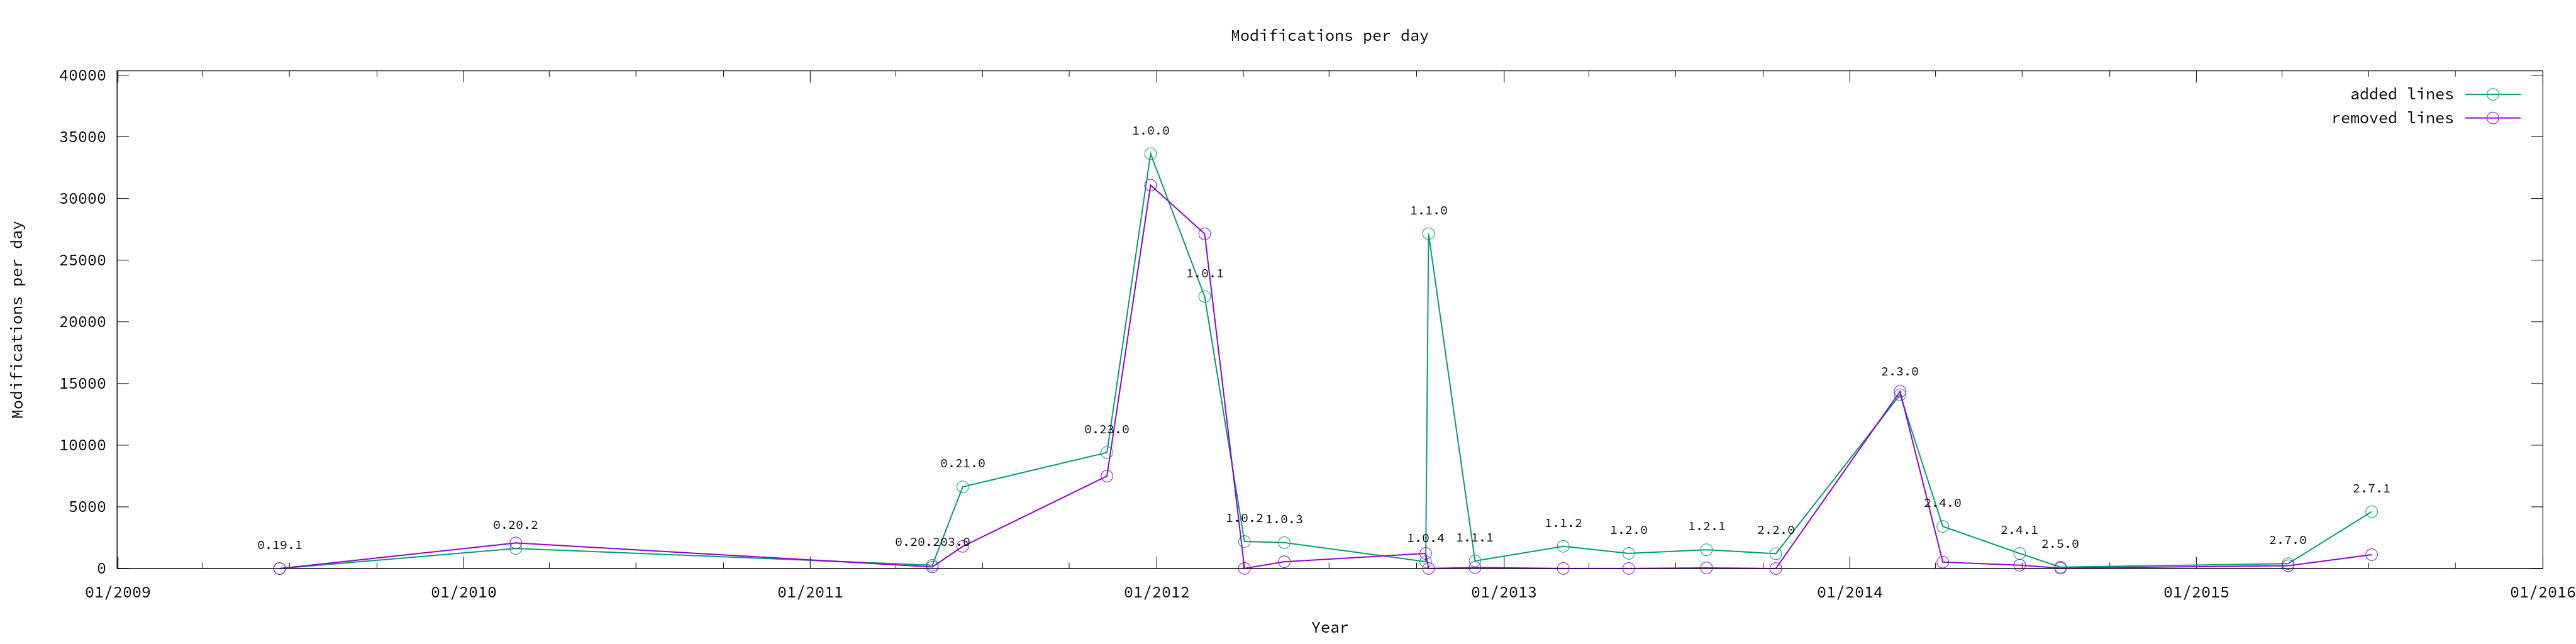
\includegraphics[width=0.7\linewidth]{figure/modifications_per_day}
	\caption{Média de modificações por dia}
	\label{fig:modificationsperday}
\end{figure}


A Figura \ref{fig:modificationsperday} mostra o número médio de adições e remoções por dia, calculados entre uma versão e sua antecessora. Nota-se que as maiores médias estão relacionadas com os maiores números de adições e remoções absolutas. Pode-se observar também que não uma tendência a invariância, e se uma grande variação das médias tanto do número de adições, quanto de remoção de linhas. O que não é surpreendente, em vista que trata-se de um projeto Open-Source, em que não há um esforço igualmente investido por todos os desenvolvedores.

Portanto, verificamos que a lei da conservação da estabilidade organizacional é falsa para o Hadoop.
%\begin{hypothesis}
%	A taxa de mudança ao longo do tempo decresce.
%\end{hypothesis}
%\begin{hypothesis}
%	A taxa de crescimento ao longo do tempo decresce.
%\end{hypothesis}
\subsection{Lei 5: Conservação da Familiaridade}
Esta lei sugere que o crescimento incremental do sistema tende a permanecer constante, porque os desenvolvedores precisam entender o código fonte e o comportamento do sistema. Como métricas, utilizamos o incremento percentual de funções e classes por versão do projeto. Assim, nossas hipóteses são:

\begin{hypothesis}
	A taxa de crescimento de funções é invariante.
\end{hypothesis}
\begin{hypothesis}
	A taxa de crescimento de classes é invariante.
\end{hypothesis}
\begin{figure}[h]
	\centering
	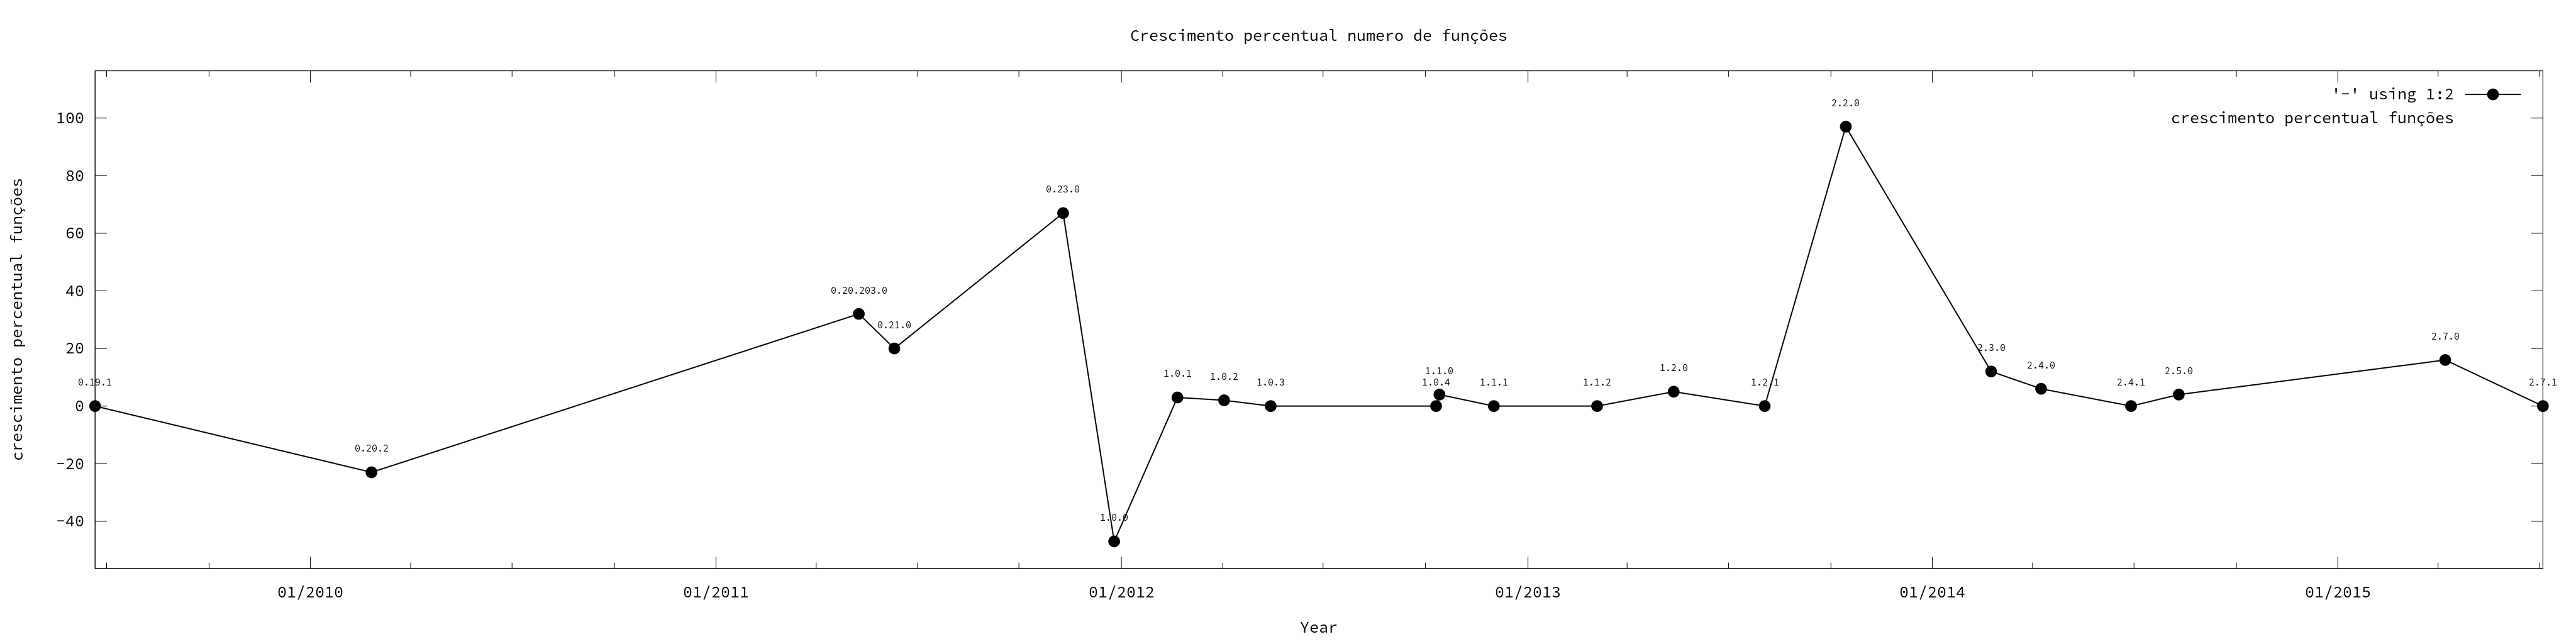
\includegraphics[width=0.7\linewidth]{figure/crescimento_percentual_funcoes}
	\caption{}
	\label{fig:crescimentopercentualfuncoes}
\end{figure}
\begin{figure}[h]
	\centering
	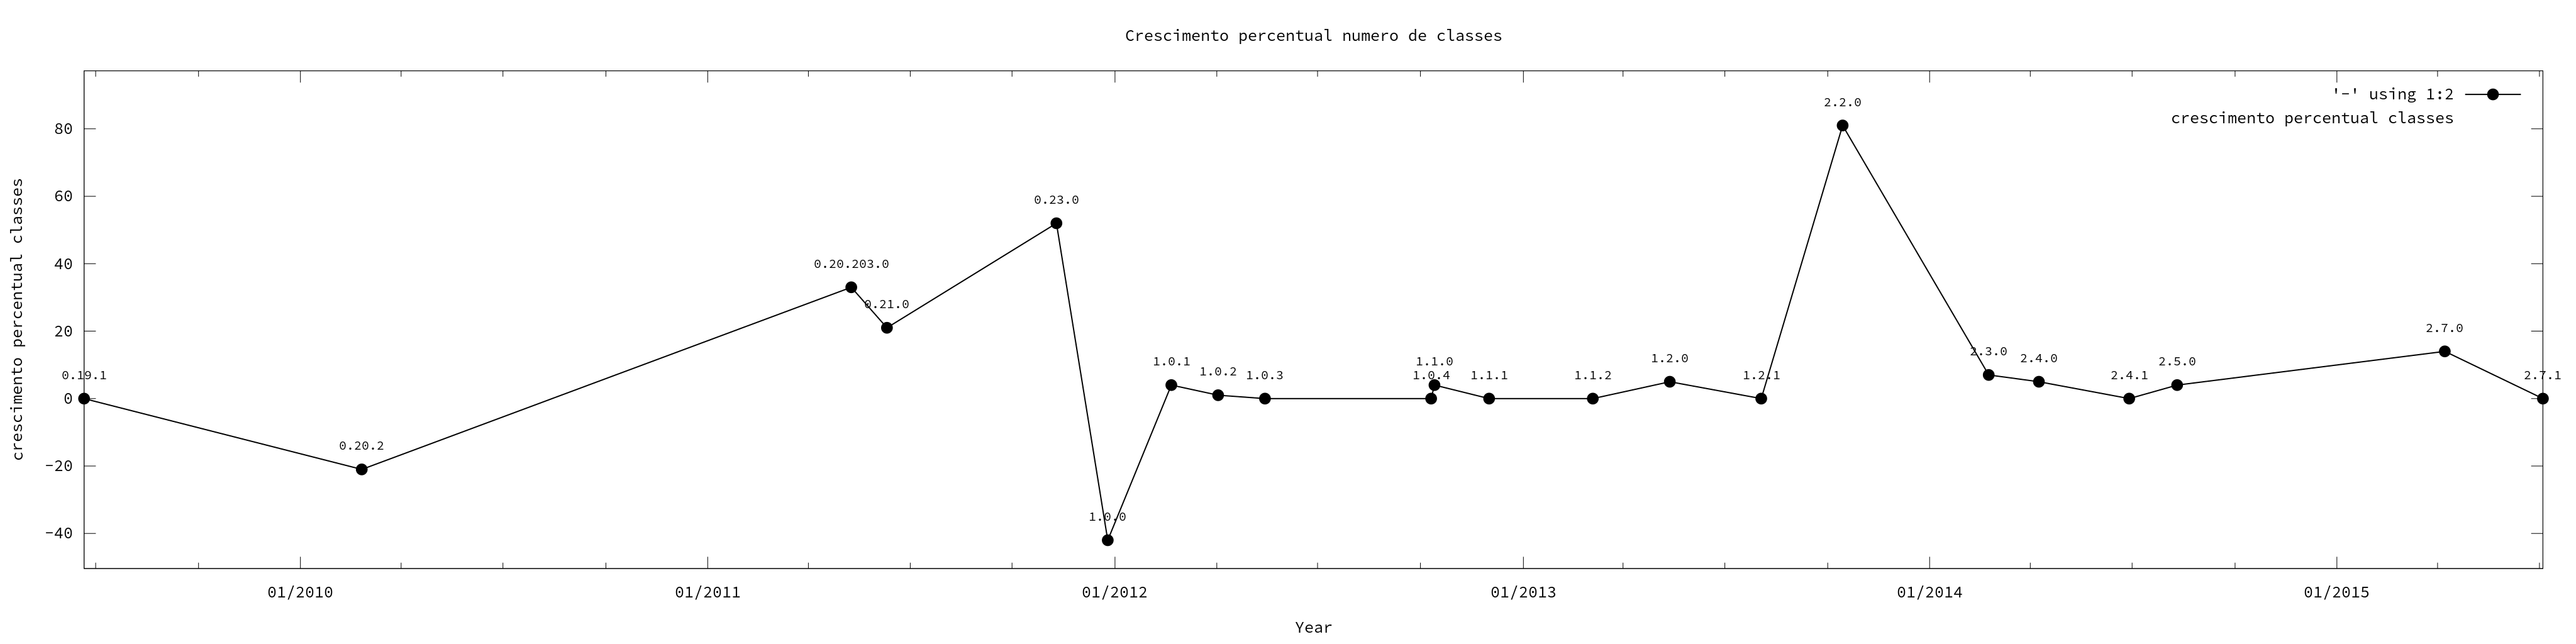
\includegraphics[width=0.7\linewidth]{figure/crescimento_percentual_classes}
	\caption{}
	\label{fig:crescimentopercentualclasses}
\end{figure}

As Figuras \ref{fig:crescimentopercentualfuncoes} e \ref{fig:crescimentopercentualclasses} representam o crescimento percentual de funções e classes, respectivamente. Assim como previsto por Lehman\cite{lehman1996laws}, versões que adicionam grandes mudanças são seguidas por lançamentos menores. Porém, ambos os indicadores mostram grande variação na adição de modificações, invalidando nossas hipóteses.

Portanto, a lei de conservação da familiaridade é falsa para o Hadoop.
\subsection{Lei 6: Crescimento Contínuo}
De acordo com esta lei, um programa deve ser constantemente incrementado ao longo do tempo para satisfazer usuários. Aqui, "crescimento" é interpretado como o tamanho do software. O tamanho pode também ser utilizado ou indicador de funcionalidade, assumindo-se que código adicional é escrito para a criação de novas funcionalidades.

Tal lei pode ser validada calculando métricas de tamanho (como número de módulos) e observando sua evolução com o tempo, assim como usado por Lehman e outros estudos\cite{lehman1980programs, lehman1985program,neamtiu2013towards}. Várias métricas podem ser utilizadas para descrever o tamanho de um software. Para o objeto de nossa análise, utilizamos linhas de código executáveis(isto é, não em branco e não comentadas), número de funções e classes para descrever o crescimento do projeto.
Portanto, nossas hipóteses são:
\begin{hypothesis}
	O número de linhas de código cresce com o tempo.
\end{hypothesis}
\begin{hypothesis}
	O número de classes cresce com o tempo.
\end{hypothesis}
\begin{hypothesis}
	O número de funções cresce com o tempo.
\end{hypothesis}

\begin{figure}
	\centering
	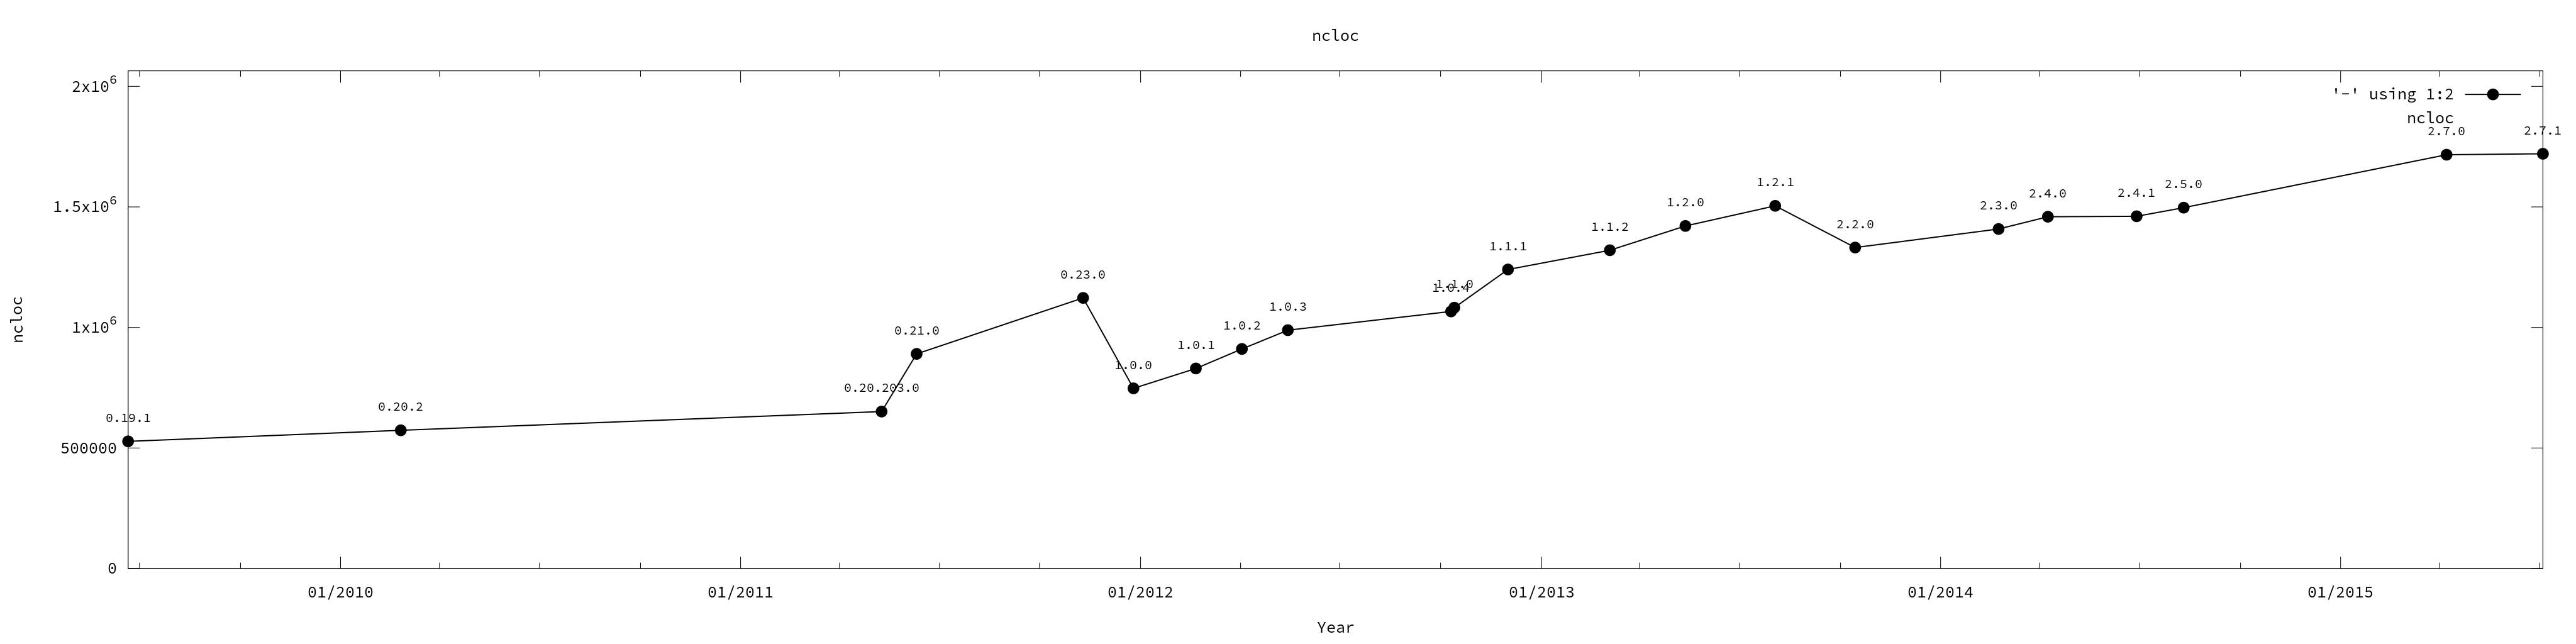
\includegraphics[width=0.7\linewidth]{figure/ncloc}
	\caption{Crescimento em Linhas}
	\label{fig:lines}
\end{figure}

As Figuras \ref{fig:function_growth}, \ref{fig:classes_growth} e \ref{fig:lines} mostram o crescimento em número de funções, classes e linhas de código, respectivamente. Com poucas exceções ao longo da sua evolução, observa-se que o Hadoop apresenta uma tendência de crescimento tomando toda seu histórico como referência, confirmando nossas hipóteses. 

Logo, podemos afirmar que a lei de crescimento contínuo é confirmada para o Hadoop.



\subsection{Lei 7: Qualidade Decrescente}

Esta lei estipula que com o tempo, a qualidade do software parece degradar-se, a não ser que medidas sejam tomadas para conter tal fenômeno. Por qualidade de código nos limitamos nossas observações a manutenibilidade de código em questão, mensurada através da dívida técnica do \textit{software}.

Assim, nossas hipóteses são:
\begin{hypothesis}
	A dívida técnica total cresce com o tempo.
\end{hypothesis}
\begin{hypothesis}
	A dívida técnica relativa total cresce com o tempo.
\end{hypothesis}
\begin{figure}[h]
	\centering
	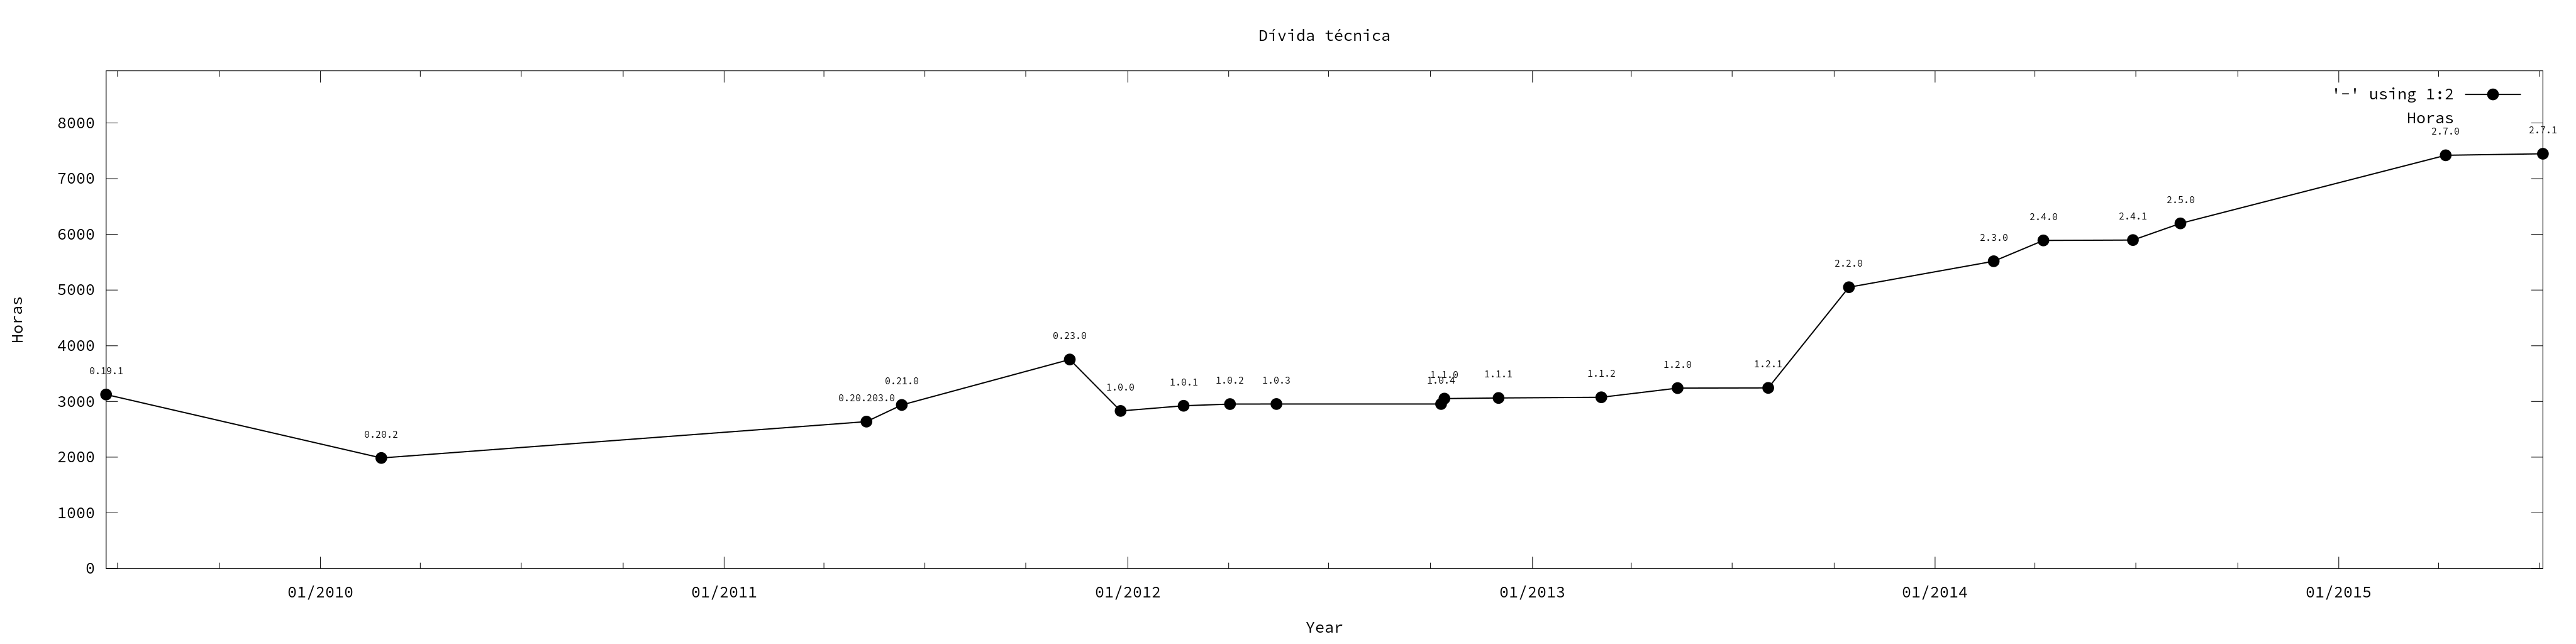
\includegraphics[width=0.7\linewidth]{figure/Horas}
	\caption{Dívida técnica total em horas}
	\label{fig:horas}
\end{figure}

As Figuras \ref{fig:horas} e \ref{fig:sqaledebtratio} a dívida técnica total e a razão da dívida técnica, respectivamente. A razão da dívida técnica calcula a razão entre o total da dívida técnica do projeto, sobre o esforço total para a criação do projeto do zero. O Sonarqube, classifica sistemas com a razão menor do que 5\% como a melhor estado para o estado interno do código. 
\begin{figure}[h]
	\centering
	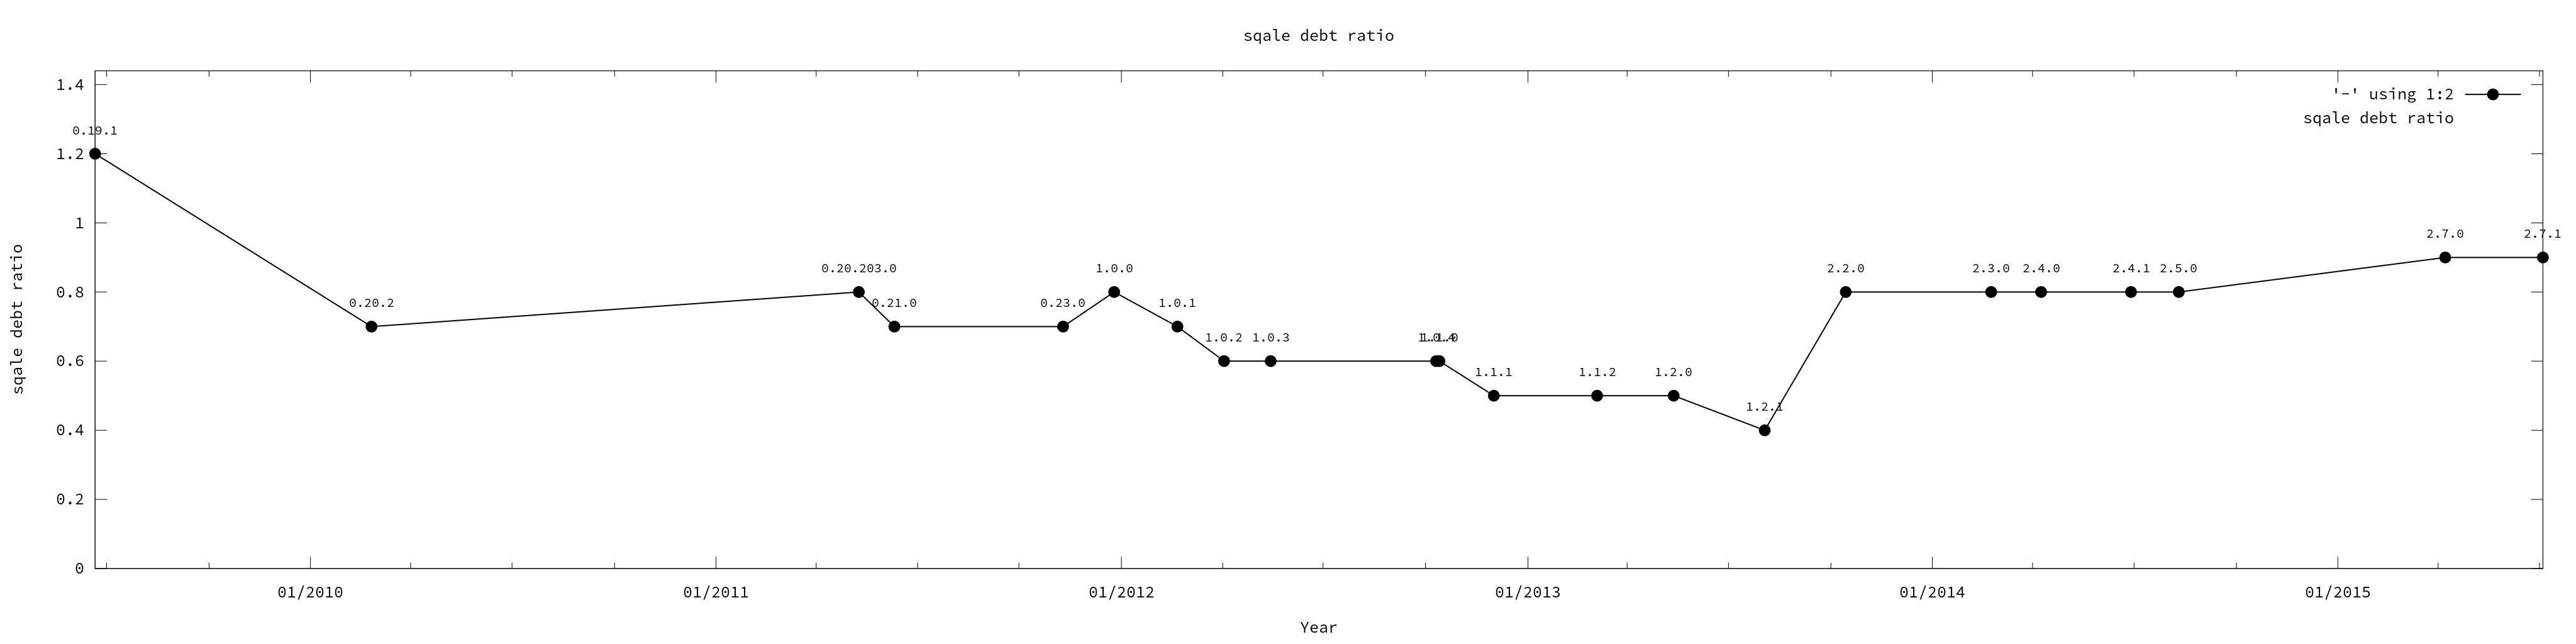
\includegraphics[width=0.7\linewidth]{figure/sqale_debt_ratio}
	\caption{Razão da dívida técnica}
	\label{fig:sqaledebtratio}
\end{figure}
Como apresentado, mesmo que a dívida técnica aumente com o tempo, a razão segue em declínio caracterizando que o código adicionado não é de baixa qualidade, e que há um esforço contínuo para resolução de defeitos.

Portanto, concluímos que a lei da qualidade decrescente não está confirmada para o Hadoop.

%\subsection{Lei 8: Sistema de Realimentação}
%
%\begin{hypothesis}
%	O número de módulos: $\alpha\sqrt[3]{RSN} $
%\end{hypothesis}
%\begin{hypothesis}
%	O número de módulos cresce com o tempo.
%\end{hypothesis}
%\begin{hypothesis}
%	O número de funções cresce com o tempo.
%\end{hypothesis}
%

\section{Discussão}


